\documentclass[12pt,a4paper]{article}
%-----------------------------------------------
%PACOTES
%-----------------------------------------------
\usepackage[utf8]{inputenc}
\usepackage[brazil]{babel}
\usepackage[T1]{fontenc}
\usepackage{amsmath}
\usepackage{amsfonts}
\usepackage{amssymb}
\usepackage{graphicx}
\usepackage[onehalfspacing]{setspace} %Espaçamento de 1,5.
\usepackage[left=3cm,right=2cm,top=3cm,bottom=2cm]{geometry}
\usepackage[T1]{fontenc} %Possibilita copiar o texto e colar em outro editor mantendo a formatação.
\usepackage{verbatim} %Possibilita comentar blocos de texto.
\usepackage[pdftex]{hyperref} %Para inserir links.

%-----------------------------------------------
%INFORMAÇÃO PARA A PÁGINA DE TÍTULOS
%-----------------------------------------------
\author{Discente Fernando Bispo}
\title{\textbf{Relatório Técnico do Sistema de Avaliação das Disciplinas do Bacharelado em Estatística da UFBA}}
\date{}
%\raggedbottom
%-----------------------------------------------
%INÍCIO DO DOCUMENTO
%-----------------------------------------------
\begin{document}

\maketitle
%\rule{0.95\textwidth}{0.5mm}

\begin{abstract} %Resumo (abstract)
\textit{
Relatório técnico do Questionário de Avaliação das Disciplinas, submetido aos discentes nos anos letivos 2018.1 e 2018.2.\\
Neste relatório são apresentadas as análises e os principais resultados obtidos do instrumento de avaliação submetido.
}
\end{abstract}

\section{Introdução}

O Sistema de Avaliação do Bacharelado em Estatística - SABE do Departamento de Estatística - DEst foi iniciado em 2018 com o intuito de coletar informações dos alunos do curso Bacharelado em Estatística da Universidade Federal da Bahia - UFBA.\\
 Os dados foram coletados por meio de questionário eletrônico encaminhado através de e-mail com o seguinte link para acesso: \url{http://www.mwstat.com/ledufba/sabe_dis/}. Foram solicitados Matrícula e CEP para identificação do respondente.
O questionário aplicado (Anexo 1) foi composto por 12 questões, dentre estas 10 relativas a Avaliação da Disciplina que se propõe a avaliar o docente, sua didática, meios de aplicação do conteúdo e métodos de avaliação e 2 destinadas a Autoavaliação, com a proposta de identificar o comprometimento do aluno perante a disciplina cursada. 
No intuito de avaliar cada disciplina em que estava matriculado, o aluno respondeu ao questionário o número de vezes que compreendesse a quantidade dessas disciplinas matriculadas, ou seja, os alunos responderam o questionário mais de uma vez. Ao todo houveram 27 respondentes representando um total de 154 respostas sendo 24 respondentes no ano letivo 2018.1 que representou um total de 96 respostas/disciplinas avaliadas e 15 respondentes no ano letivo 2018.2 que representou um total de 58 respostas/disciplinas matriculadas. Entende-se que parcela dos respondentes pertencentes ao semestre 2018.1 também responderam o questionário no semestre 2018.2, sendo estes identificados pelo número de matrícula, justificando assim o total de respondentes não corresponder a soma de respondentes nos dois semestres letivos.
O campo denominado por outros representa os alunos que foram reprovados por falta e os alunos que trancaram disciplinas, pois, suas respostas não foram consideradas em virtude da natureza da reprovação, totalizando 03 respondentes o que corresponde a 11,11\% do total de respondentes ao questionário, em que estes respondentes foram reprovados por falta ou trancaram um total de 09 disciplinas que representam 5,84\% do total das avaliações realizadas.
Foi utilizada a Escala Likert de 5 pontos de satisfação a fim de se obter a resposta que mais traduz a opinião do respondente.

\begin{comment}

teste de comentário
\end{comment}

\section{Resultados e Discussão}
\subsection{Disciplinas}
Dentre as disciplinas ofertadas pelo curso, foram listadas das respostas dos alunos um total de 35 disciplinas distintas, estando estas dispostas em 4 grupos conforme o departamento a que pertencem, sendo estes DCC - Departamento de Cência da Computação, DMat - Departamento de Matemática, DEst - Departamento de Estatística e Outros representando o conjunto de disciplinas menos frequentes, conforme Figura 1.

\begin{figure}[!h]
\centering
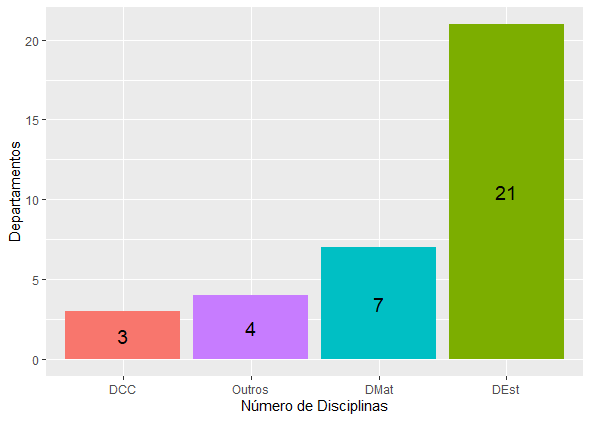
\includegraphics[scale=0.7]{Imagens/G1.png}
\caption{Quantidade de disciplinas por departamento.}
\end{figure}

No semestre 2018.1 os respondentes estavam matriculados em 24 disciplinas em que as disciplinas MAT198, MATB59, MAT229 e MATD45 foram as que tiveram maior quantitativo de avaliações dos alunos e consequentemente maior quantitativo de alunos matriculados, com 8 avaliações nas duas primeiras listadas representando 5,19\% do total de respostas ao questionário e 7 avaliações nas duas últimas listadas representando 4,55\% do total de respostas ao questionário. No semestre 2018.2 os respondentes estavam matriculados em 23 disciplinas, em que as disciplinas com maior quantidade de avaliações dos alunos e
consequentemente maior quantidade de alunos matriculados foram MAT174, MAT186 e MATD42 com 5 avaliações nas duas primeiras representando 3,25\% do total de respostas ao questionário e 4 avaliações na última representando 2,60\% de respostas ao questionário


























\end{document}